\documentclass{fose2016}           % for pLaTeX2e
%\documentclass[english]{fose2016} % for English papers
%\documentclass[ascii]{fose2016}   % for ASCII pTeX 

\usepackage[dvipdfmx]{graphicx}
%\usepackage{epsfig}

\title{依存関係の向きを考慮したファイルの変更時間への影響分析}
\etitle{}% TODO dependency file, vector, develop time, impact analysis
\author{上田 裕己}{Ueda Yuki, 島根大学}
\author{神谷 年洋}{Kamiya Toshihiro, 島根大学}

\begin{document}



\maketitle

\begin{abstract}
大規模なソフトウェア開発では多くのファイルからソフトウェアが成り立っている.
そのため,あるファイルを変更した場合ほかのファイルにも影響を及ぼす.

既存研究では依存関係がソフトウェアの品質や開発者の経験に影響を与えることがわかっている.

本研究では,変更されたソースコードの依存関係の依存の向きに着目して,依存関係をもつファイルが次に変更されるまでの期間への影響を調査した.
 
実験結果から変更されているソースコードに依存関係の向きや変更を行った人物によって開発期間に大きく影響を与えることが分かった.
  

\end{abstract}

\begin{eabstract}

\end{eabstract}

%はじめに
\section{はじめに} 
% 現在開発者の経験を図るために多くの研究で開発者がいままでに変更したファイルが利用されている.
ソフトウェア開発において開発者に対してそれぞれ適した仕事を割り振ることは開発期間の短縮や不具合の回避に対して重要である.

Bird\cite{Bird}らは専門レベルという開発者があるファイルに対してどれだけ詳しいかという度合いによってソフトウェアの故障率に影響を与えるという研究を行った.
これにより,ソフトウェアプロジェクトの管理者は問題に対して最適な開発者を割り当てることができる.

しかし,対象ファイル群が依存する他のファイル群(以降,依存ファイル群)に対する専門レベルは考慮されていない.これは,変更が行われたファイルと依存関係にあるファイルに対して十分な検査が行えず,不具合を見逃す恐れがある.


そのため,本論文では変更されたファイルに対して依存関係のあるファイルが変更されるまでの時間の間隔(以降,変更時間間隔(単位:日))への影響について調査を行った.

ある変更が行われてから,早い変更時間間隔で変更が行われるファイルには, 不具合が発生やリファクタリングが起きていると考えられる.% そういった文献を探したほうがよさそう(ealy fix)

変更時間間隔を調査することにより,どのような依存関係のあるファイルに開発者が注目すればいいのかが,わかることが期待される.

そのために変更が行われたファイルに対して,プロジェクト内のすべてのファイルがどのような依存関係を持っているのか6つに分類を分けそれぞれの変更時間間隔への影響を調査する.

また, プロジェクトに権限を持っている人物による変更であることによる変更時間間隔への影響を調査するために,同じ人物が変更した場合,マージとなった変更の場合でも同様の調査を行った.


本論文では\ref{関連研究}章で関連研究について書き\ref{調査方法}章で調査方法,\ref{実験結果}章で実験の結果,\ref{考察}章で実験結果についての考察,\ref{妥当性の検証}章では実験の妥当性についての検証,最後に\ref{まとめ}章でまとめを行う.


%関連研究
\section{関連研究}\label{関連研究}

Briand\cite{Briand}らは依存関係が変更までの時間に影響を与えることを調査した.

この研究では,変更されたファイルに対して依存しているファイルのみを調査している.

この問題点は変更されたファイルに対して依存されているファイルに対して調査が行われていない.
これにより,同じ機能を重複して実装したり, 機能を抽象化するさいの変化を終えていない可能性がある.


\subsection{変更波及解析}
変更波及解析とは



そこで,我々は依存されているファイルを同様に調査することによって依存関係の向きも考慮した.


% リサーチクエスチョン
\section{リサーチクエスチョン(RQ)}\label{リサーチクエスチョン}
以下の項目について調査を行う.
\begin{itemize}
\item RQ1:変更されたファイルに依存関係のあるファイルが変更されるまでの時間は依存関係のないファイルより短くなる
\item RQ2:依存関係があるファイル(fがgに依存)の変更において、gが変更されたあとfが変更時間間隔は、fとgの開発者が同じ場合には、異なる場合よりも,短くなる
\item RQ3::依存関係があるファイル(fがgに依存)の変更において、gが変更されたあとfが変更時間間隔は、fのコミットが複数のブランチのマージとなったコミットである場合には,異なる場合よりも,長くなる
\end{itemize}
% RQ1
\subsection{RQ1:変更されたファイルに依存関係のあるファイルが変更されるまでの時間は依存関係のないファイルより短くなる}
依存関係に種類を定義することによってどの種類がファイルの変更時間間隔に影響を与えるのか調査を行った..

ここでは,以下のことについて調査を行う.
\begin{enumerate}
\item RQ1-1ファイルfがファイルgに依存するとき、gが変更されたあとfが変更されるまでの時間は、依存関係がないファイルと比較して短い
\item RQ1-2 ファイルfがファイルgに依存するとき、fが変更されたあとgが変更されるまでの時間は、依存関係がないファイルと同じである
\end{enumerate}

また,本研究ではソースコードのうち以下のような記述を依存関係として扱う.
変更が行われたファイルに対して以下の例のような記述が存在した場合,クラスAを定義しているファイルに依存しているとする.

\begin{itemize}
\item 参照による代入や呼び出し,定義(例:ClassA a = new ClassA())
\item 継承 (例: ClassB extends ClassA)
\end{itemize}

\subsubsection{依存関係の分類}
依存関係があるファイルにも依存関係の方向や間接的な依存関係をもつものを考慮するためにプロジェクト内のすべてのファイルを表\ref{tab:依存関係の分類}に示したような分類に分ける.
本論文ではこの分類を依存関係の分類と呼ぶことにする.図\ref{fig:dependency}に依存関係の分類についての図を用意した.

\begin{table}
\caption{依存関係の分類}
\begin{tabular}{|l|r|r|} \hline
分類名 & 概要 \\ \hline
root & 変更されたファイル \\ \hline
dependee & rootが依存するファイル \\ \hline
depender & rootが依存されるファイル \\ \hline
dependee2 & dependeeが依存するファイル \\ \hline
depender2 & dependerが依存されるファイル \\ \hline
other & 上記に当てはまらないファイル \\ \hline
\end{tabular}
\label{tab:依存関係の分類}
\end{table}

\begin{figure}[t]
\centering
\includegraphics[width=\columnwidth]{dependency.pdf}
\caption{依存関係の分類図}
\label{fig:dependency} 
\end{figure}

% RQ2
\subsection{RQ2:依存関係があるファイル(fがgに依存)の変更において、gが変更されたあとfが変更時間間隔は、fとgの開発者が同じ場合には、異なる場合よりも、短くなる}
同一人物が変更を行った場合とそうでない場合でRQ1と同じく変更時間間隔への影響を調査した.
これを調べることにより, 依存関係による影響を解決している人物はどのような依存関係に集中しているのか,
また,同じ開発者であることによって,どのような依存関係のあるファイルが影響を受けるかをRQ1と同様に調査する.

% RQ3
\subsection{RQ3:依存関係があるファイル(fがgに依存)の変更において、gが変更されたあとfが変更時間間隔は、fのコミットが複数のブランチのマージとなったコミットである場合には,異なる場合よりも,長くなる}
マージされていないコミットの場合はレビューが行われていない可能性が高い.

レビューが行われていないファイルの多くはほかの開発者に確認をされていないため信頼性が低いと考えられる.
よってマージとなるコミットはそうでないコミットよりも変更時間間隔が長くなると考えた.

ここではマージされたコミット変更ではそうでない変更の変更時間間隔を,RQ1と同様に依存関係の分類別に,比較してどのような影響があるのか調査をする.

                                                                                                                                                                                                                                                                                                                                                                                                                                                                                                                                                                                                                                                                                                                                                                                                                                                                                                                                                                                                                                                                                                                                                                                                                                                                                                                                                                                 % 調査方法
\section{調査方法}\label{調査方法}

\subsection{調査対象のデータセット}
GitHub上のeclipseプロジェクトの中で最もstar数が多かったvert.vプロジェクトを調査,
vert.vプロジェクトは2013年から2016年まで変更され続け,合計2000以上のコミットが行われている.
eclipseプロジェクトには多くのオープンソースソフトウェアがあり,今後ほかのプロジェクトと比較するのに適していると考えた


\subsubsection{出力するデータセット}
csv形式で時系列とともに出力する.
出力するデータを表\ref{tab:初期データセット}に示した.


\begin{table}[htb]
\caption{出力するデータセット}
\begin{tabular}{|l|r|r|} \hline
属性名 & 概要 \\ \hline
filepass & ファイルの絶対パス \\ \hline
commitNo & HEADからのコミットの距離 \\ \hline
date & 変更が行われた日付 \\ \hline
author & 変更を行った開発者の名前 \\ \hline
kind & 依存関係の種類 \\ \hline
ismerge & マージされた後のコミットであるかどうか \\ \hline
\end{tabular}
\label{tab:初期データセット}
\end{table}

filepassとは出力するファイルのファイルパスである.
同一のcommitNoに対してその時点でのプロジェクトでのすべてのjavaファイルを出力している.
このファイルパスは一意ではなく,同じfilepassとcommitNoでもkindが別のものがある.
データ型は文字列型である.

commitNoとは最新の変更からの変更の距離を示している.データ型は数値型である.

dateとは変更が行われた日付を出力している.データ型は日付型である.

authorとは変更を行った開発者の名前を出力している.データ型は文字列型である.

kindとは依存関係の分類を出力している.データ型は文字列型である.

ismergeとはコミットがmergeされたコミットかどうかを分類しているものであり,論理型の値を得る.

図{fig:gitimage} にコミットの分類を図示する.
このうちismergeがTrueとなるのは1と2のコミットである.

\begin{figure}[t]
\centering
\includegraphics[width=\columnwidth]{git_image.pdf}
\caption{gitによるコミットの分類分け}
\label{fig:gitimage} 
\end{figure}


これらの情報をもとに変更時間間隔を求める.
データ型は数値型である.

%SubCommitNoとは次に変更があるまでの変更の数である.
%データ型は数値型である.

このデータはkindがrootのもの以外に対してつけられる.

以下の手順でデータ取得を行う.
\begin{enumerate}
\item プロジェクトの状態を一つ過去のものに戻す.
\item その状態のプロジェクト内のファイルの情報,をXML形式で出力する.
\item 生成されたXMLファイルから依存関係を求める.
\item その状態のプロジェクト内のすべてのファイルの情報,表\ref{tab:初期データセット}をcsvファイルに出力する.
\item すべての過去の変更を調べるまで1に戻る
\end{enumerate}
これにより得られたデータ量は141MGとなった.

% RQ 利用したツール
\subsection{データ収集に利用したツール・サービス}
% git
\subsubsection{バージョン管理システム, git}
バージョン管理システムとはファイルの変更の履歴を保存するためのシステムである.
現在多くのソフトウェアではバージョンコントロール管理システムが利用されている.
今回調査を行ったvert.vプロジェクトも同様にバージョン管理システムの一つであるgitで管理されている.

gitなどの分散型のバージョン管理システムでは,多くの開発者が一つのソフトウェアを変更していても,変更の重複を防ぐことができる.

gitで利用されているものにブランチがある.
ブランチは履歴の流れを分岐して記録していくためのものであり,同じプロジェクトの中で複数の変更を同時に進めていくことを目的としている.
このブランチをmasterという主となるブランチに対して行われたマージを''マージとなるコミット''とする.

% GitHub
\subsubsection{GitHub}
さまざまなオープンソースソフトウェアを管理しているサービスである.
これを利用して認可のあるプロジェクトや開発者の状況を確認したり,ほかの開発者と議論をすることができる.

プロジェクト外の開発者もGitHubにあるソースコードを別のブランチとして変更し,その変更を投稿することができる.
GitHub内で変更が投稿された時,コードレビューという,変更を行った開発者とは別の開発者によるコードの査読が行われる.
このコードレビューで有用と判断された変更はmasterにマージされる.


% doxygen
\subsubsection{doxygen}
ソースコード解析ツール.XML形式でファイルごとに宣言や状況などを出力することができる.
今回の研究では依存関係を検出するために利用した.



%実験結果
\section{実験結果}\label{実験結果}
依存関係の分類別,また同じ開発者が変更を行っているか,マージとなるコミットであるかによって依存関係を持つファイルの変更時間間隔を出力した.

%実験・RQ1
\subsection{RQ1:変更されたファイルに依存関係のあるファイルが変更されるまでの時間は依存関係のないファイルより短くなる}
図\ref{fig:subdate}はそれぞれ依存関係別にみた依存関係の検出から変更時間間隔を箱ひげ図で出力したものである.  

\begin{figure}
\centering
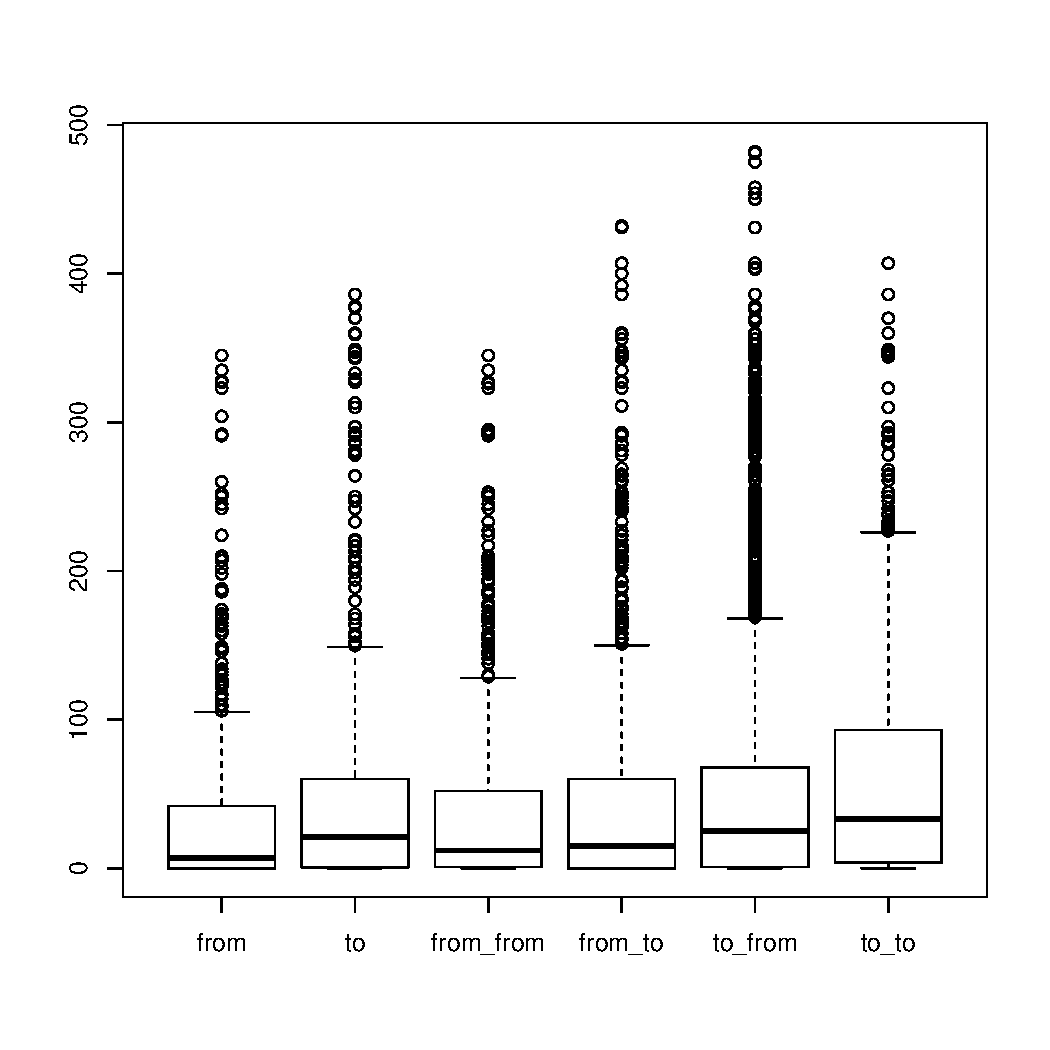
\includegraphics[width=0.5\columnwidth]{date.pdf}
\caption{依存関係の分類ごとの変更時間間隔}
\label{fig:subdate} 
\end{figure}


%ここでのp-value検定の表もだす


図\ref{fig:subdate}から依存関係別で優位に差があることが判明した.
よって以下のRQ2,RQ3でも,この依存関係の分類を用いることにする.


%実験・RQ2
\subsection{RQ2:依存関係があるファイル(fがgに依存)の変更において、gが変更されたあとfが変更時間間隔は、fとgの開発者が同じ場合には、異なる場合よりも、短くなる}
依存関係をもつファイルを同じ開発者が変更した場合の変更時間間隔への影響を調査した.
図の\label{fig:author_true_subdate} は同じ開発者が変更した場合の変更時間間隔を出力している.
また,図の\label{fig:author_false_subdate} は異なる開発者が変更した場合の変更時間間隔を出力している.

\begin{figure}
\centering
\begin{minipage}{0.49\columnwidth}
\centering
\includegraphics[width=\columnwidth]{author_date_TRUE.pdf}
\caption{同じ開発者の依存関係の分類ごとの変更時間間隔}
\label{fig:author_true_subdate} 
\end{minipage}
\begin{minipage}{0.49\columnwidth}
\centering
\includegraphics[width=\columnwidth]{author_date_FALSE.pdf}
\caption{異なる開発者の依存関係の分類ごとの変更時間間隔}
\label{fig:author_false_subdate} 
\end{minipage}
\end{figure}


%実験・RQ3
\subsection{RQ3:依存関係があるファイル(fがgに依存)の変更において、gが変更されたあとfが変更時間間隔は、fのコミットが複数のブランチのマージとなったコミットである場合には,異なる場合よりも,長くなる}
マージとなるコミットの変更時間間隔の影響を調査した.
図の,\label{fig:merge_true_subdate} はマージとなるコミットの変更時間間隔を出力している.
また,図の\label{fig:merge_false_subdate} はマージではないコミットの変更時間間隔を出力している.

\begin{figure}
\centering
\begin{minipage}{0.49\columnwidth}
\centering
\includegraphics[width=\columnwidth]{merge_date_TRUE.pdf}
\caption{マージとなるコミットの依存関係の分類ごとの変更時間間隔}
\label{fig:merge_true_subdate} 
\end{minipage}
\begin{minipage}{0.49\columnwidth}
\centering
\includegraphics[width=\columnwidth]{merge_date_FALSE.pdf}
\caption{マージではないコミットの依存関係の分類ごとの変更時間間隔}
\label{fig:merge_false_subdate}
\end{minipage}
\end{figure}


%考察
\section{考察}\label{考察}

%考察 RQ1
\subsection{RQ1:変更されたファイルに依存関係のあるファイルが変更されるまでの時間は依存関係のないファイルより短くなる}
図\ref{fig:subdate}について考察する.

最も開発期間が長いものがotherであることから依存関係があるものは依存関係の向きや長さを問わず早く変更される傾向にあると考えられる.


dependerやdepender2からわかるように変更されたファイルに依存しているファイルが早く変更される傾向にあることが分かった.
すべてのファイルの変更されるまでの日付の中央値は25日なのに対してdependerは約5日で変更される.
このことから依存関係の距離よりも依存関係の向きが開発機関に影響を与えることが分かった.
基本的に変更によって影響を受けるものは変更されたファイルに依存関係をもつファイルであることが予測できるため,妥当な結果であるといえる.

しかしdependerやdepender2もotherよりは開発期間が短くなることから, 変更されたファイルに対して依存されているファイルも影響を受けることが分かった.
変更する理由としては変更後に同じ機能を実装した場合や必要なデータが増えたことが予測される.
自然言語処理やコードクローンの調査を行うことによってファイルや変更の種類について発見が期待される.


以上から,影響があるのは順に依存関係の向き,依存関係の距離が関係していることがわかる.


% 考察 RQ2
\subsection{RQ2:依存関係があるファイル(fがgに依存)の変更において、gが変更されたあとfが変更時間間隔は、fとgの開発者が同じ場合には、異なる場合よりも、短くなる}
図\ref{fig:author_true_subdate} と\ref{fig:author_false_subdate} について考察する

同じ人物が変更した場合と比較し,違う人物が変更したファイルは全体的に中央値が高い結果になっている.
dependee2とotherを比較した場合,違い人物が変更した場合には大きな差がないのに対して,同じ人物が変更した場合は20日近く差があることが分かった.

同じ人物が変更した場合に中央値が下がることに関して考えられることは,同じ開発者が変更したコミットの大部分は同時に変更をしたものである.
多くの開発者が不具合がでないように他の依存関係のあるファイルを変更するので妥当な結果といえる.

別の開発者が変更をした場合にはdependee2とotherに対して大きく差がでる.

これは同じパッケージに入っているために影響がでることが考えられる.

%考察 RQ3
\subsection{RQ3:依存関係があるファイル(fがgに依存)の変更において、gが変更されたあとfが変更時間間隔は、fのコミットが複数のブランチのマージとなったコミットである場合には,異なる場合よりも,長くなる}
図\ref{fig:merge_true_subdate} と\ref{fig:merge_false_subdate} について考察する

マージされたコミットほど変更されるタイミングが遅くなる.
また,マージされていないコミットではdependee2とotherとの差がないことがわかった.


mergeされたコミットの場合mergeされていないコミットと比較して次に変更される時期が遅くなる傾向がある.
以下はその理由を考察した.
\begin{enumerate}
\item レビューを通してから変更を適用するために信頼性が高く,変更の必要がなくなる
\item mergeされ終わり, 作業が減る
\item 変更を行ったのがコアコミッターではないため不具合があったとしても修正に時間がかかる
\end{enumerate}

特にmergeされたコミットではdependee2はotherと中央値が近い数値を出している.
以下に理由について考察した.

\begin{enumerate}
\item 外部からの変更ではあまり抽象的になりがちなファイルを変更しづらい
\item 絶対数が少ないため, 変更されにくい
\end{enumerate}

% 妥当性の検証
\section{妥当性の検証}\label{妥当性の検証}
次に,妥当性について検証を行う.

\subsection{プロジェクト固有の特性}
今回の実験で用いたプロジェクトはオープンソースである,eclipseのプロジェクトである.
ほかのオープンソースプロジェクトや商業ソフトウェアで,同様結果が得られるとは限らない.
特にソフトウェアの規模によっては開発者の違いや全体的な開発期間に影響があることが予測される.

\subsection{依存関係の扱いについての影響}
依存関係についての調査では継承や参照もすべて同じ依存関係であるとした.
これらを同じように扱うことで別のデータに偏りが発生した可能性がある.
例えば継承関係については

% まとめ
\section{まとめ} \label{まとめ}
本研究では,ファイルの依存関係が変更時間間隔に与える影響について調査した.
その結果,依存関係の向きや距離によって時間間隔はが変化し,
同一の開発者によって変更が行われた場合のようにどのようなファイルでも変更時間間隔が短くなる要素と
,マージではないコミットの場合に依存関係のあるファイルに対して特に変更時間間隔が短くなる要素があることが分かった.

ここから,マージではないコミットほど早く変更されやすいことから,レビューを行わない変更の場合は特に依存関係に注意をする必要がある.
今回は一つのオープンソースプロジェクトのみを調査した.ほかのプロジェクトでも同じような傾向がみられるか調査する必要がある.

\section*{謝辞}
本研究はJSPS科研費16K12412の助成を受けたものである.


\begin{thebibliography}{10}
\bibitem{Ryder}
Ryder, Barbara G., and Frank Tip. "Change impact analysis for object-oriented programs." Proceedings of the 2001 ACM SIGPLAN-SIGSOFT workshop on Program analysis for software tools and engineering. ACM, 2001.
\bibitem{Briand}
Briand, L. C., Labiche, Y., O’Sullivan, L., and Sówka, M. M. (2006). Automated impact analysis of UML models. Journal of Systems and Software, 79(3), 339-352.
\bibitem{Canfora}
 Canfora, G., Ceccarelli, M., Cerulo, L., and Di Penta, M. (2010, September). Using multivariate time series and association rules to detect logical change coupling: An empirical study. In Software Maintenance (ICSM), 2010 IEEE International Conference on (pp. 1-10). IEEE.
\bibitem{Budgen}
Budgen, D., Burn, A. J., Brereton, O. P., Kitchenham, B. A., and Pretorius, R. (2011). Empirical evidence about the UML: a systematic literature review. Software: Practice and Experience, 41(4), 363-392.
\bibitem{Bird}
Bird, Christian, et al. "Don't touch my code!: examining the effects of ownership on software quality." Proceedings of the 19th ACM SIGSOFT symposium and the 13th European conference on Foundations of software engineering. ACM, 2011.
\bibitem{Balachandram}
V. Balachandran: Reducing Human Effort and Improving Quality in Peer Code Reviews using Automatic Static Analysis and Reviewer Recommendation, ICSE'13, pp. 931-940, 2013.
\bibitem{Thongtanunam}
Patanamon Thongtanunam, Chakkrit Tantithamthavorn, Raula Gaikovina Kula, Norihiro Yoshida, Hajimu Iida, Ken-ichi Matsumoto: Who Should Review My Code? A File Location-Based Code-Reviewer Recommendation Approach for Modern Code Review, 22nd IEEE International Conference on Software Analysis, Evolution, and Reengineering, 2015.
\bibitem{Thongtanunam2}
Patanamon Thongtanunam and Shane McIntosh and Ahmed E. Hassan and Hajimu Iida: Revisiting Code Ownership and Its Relationship with Software Quality in the Scope of Modern Code Review, Proc. of the International Conference on Software Engineering (ICSE), 2016
 \end{thebibliography}

\end{document}
